\documentclass{beamer}
\usepackage[outputdir=build]{minted}
\usepackage[skins,minted,breakable]{tcolorbox}
\usepackage[spanish]{babel}
\usepackage{subcaption}
\usepackage{multicol}
\graphicspath{ {../img/} {../../LaTeX/img/} {/home/csp98/latex/img/}}
\selectlanguage{spanish}
\newtheorem{ppio_invarianza}{Principio de Invarianza}
\usepackage[utf8]{inputenc}
\usetheme{PaloAlto}
\setbeamerfont{section in sidebar}{size=\fontsize{2}{4}\selectfont}
\setbeamerfont{subsection in sidebar}{size=\fontsize{2}{3}\selectfont}
\setbeamerfont{subsubsection in sidebar}{size=\fontsize{2}{2}\selectfont}

\setbeamerfont{section in toc}{size=\footnotesize}
\setbeamerfont{subsection in toc}{size=\scriptsize}
\setbeamerfont{subsubsection in toc}{size=\tiny}




\title{Práctica 2}
\date{6 de abril de 2018}
\subtitle{El elemento en su posición}

\author{María Jesús López Salmerón \\ Nazaret Román Guerrero \\ Laura Hernández Muñoz \\ José Baena Cobos  \\ Carlos Sánchez Páez}

\makeatletter
  \setbeamertemplate{sidebar \beamer@sidebarside}%{sidebar theme}
  {
    \beamer@tempdim=\beamer@sidebarwidth%
    \advance\beamer@tempdim by -6pt%
    \insertverticalnavigation{\beamer@sidebarwidth}%
    \vfill
    \ifx\beamer@sidebarside\beamer@lefttext%
    \else%
      \usebeamercolor{normal text}%
      \llap{\usebeamertemplate***{navigation symbols}\hskip0.1cm}%
      \vskip2pt%
    \fi%
}%
\makeatother

\subject{Algorítmica}

\AtBeginSubsection[]
{
  \begin{frame}<beamer>{Índice}
    \tableofcontents[currentsection,currentsubsection]
  \end{frame}
}

% Let's get started
\begin{document}
\centering
\begin{frame}
  \titlepage
\end{frame}

\begin{frame}{Índice}
  \tableofcontents
  % You might wish to add the option [pausesections]
\end{frame}


\section{Cálculo de la eficiencia empírica}

\subsection{Diseño de algoritmos}

\begin{frame}[fragile]{Clásico}
\begin{minted}[fontsize=\small]{c++}
  int elementoEnSuPosicion(const vector<int> v) {
  	for (int i = 0; i < v.size() ; i++)
  		if (v[i] == i)
			return i;
	return -1;
  }
\end{minted}  
\end{frame}

\begin{frame}[fragile]{Divide y Vencerás}
\begin{minted}[fontsize=\footnotesize]{c++}
int elementoEnSuPosicion(const vector<int> v,
		 const int ini, const int fin) {
	if (ini == fin) {	//Caso base
		if (v[ini] == ini)
			return ini;
		else
			return -1;
	}
	else {
		int mitad = (ini + fin) / 2;
		int pos_izq = elementoEnSuPosicion
				(v, ini, mitad);
		int pos_dcha = elementoEnSuPosicion
				(v, mitad + 1, fin);
		if (pos_izq != -1)
			return pos_izq;
		else
			return pos_dcha;
	}
}
\end{minted}  
\end{frame}

\subsection{Medición de tiempos}

\begin{frame}[fragile]{Modificación de código fuente}
\begin{minted}[fontsize=\small]{c++}
  high_resolution_clock::time_point tantes;
  high_resolution_clock::time_point tdespues;
  duration<double> tiempo;
  double acumulado = 0;
  int pos;
  for (int i = 0; i < 1000; i++) {
	 tantes = high_resolution_clock::now();
	 pos = elementoEnSuPosicion(myvector);
	 tdespues = high_resolution_clock::now();
	 tiempo = duration_cast<duration<double>>
	 	        (tdespues - tantes);
	 acumulado += tiempo.count();
  }
  acumulado /= 1000;
\end{minted}
\end{frame}


\subsection{Tamaños de problema}
\begin{frame}[fragile]{Tamaños de problema}
\begin{table}[H]
\centering
\resizebox{\textwidth}{!}{%
\begin{tabular}{|c|c|c|c|}
\hline
\textbf{Algoritmo}  & \textbf{Tamaño inicial} & \textbf{Tamaño final} & \textbf{Incremento}\\
\hline
Clásico & 1.000.000 & 1.480.000 & 20.000 \\
Divide y Vencerás & 1.000 & 3.400 & 100\\
\hline
\end{tabular}
}
\end{table}
\end{frame}
\subsection{Resultados}

\begin{frame}[fragile]{Algoritmo clásico}
\begin{figure}[H]
\centering
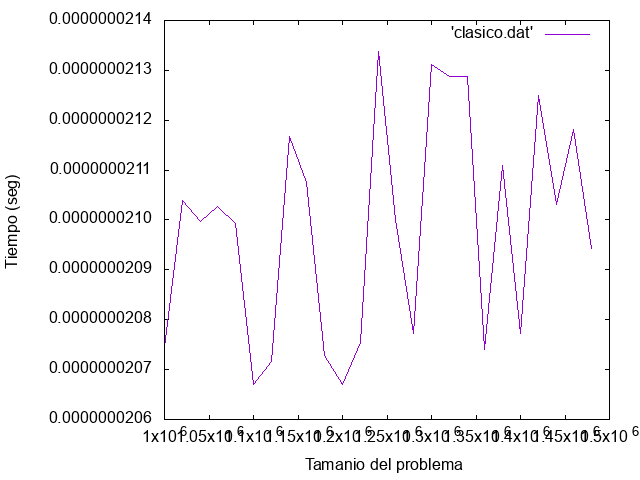
\includegraphics[scale=0.5]{clasico.png}
\end{figure}
\end{frame}

\begin{frame}[fragile]{Algoritmo Divide y Vencerás}
\begin{figure}[H]
\centering
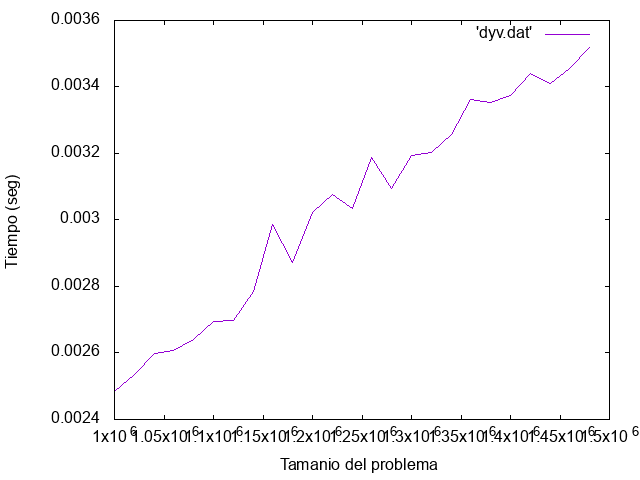
\includegraphics[scale=0.5]{dyv.png}
\end{figure}
\end{frame}

\subsection{Comparación de algoritmos}
\begin{frame}[fragile]{Comparación entre ambos algoritmos}
\begin{figure}[H]
\centering
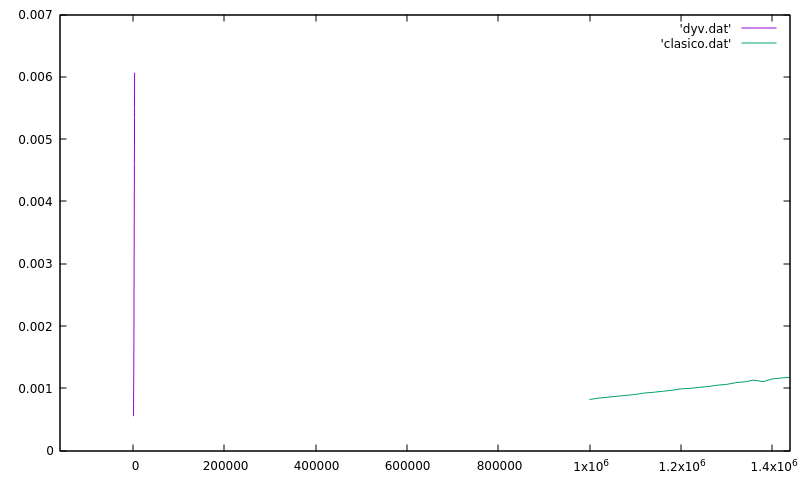
\includegraphics[scale=0.5]{empirica_ambos.png}
\end{figure}
\end{frame}

\section{Cálculo de la eficiencia híbrida}

\subsection{Errores en el cálculo de la constante oculta}
\begin{frame}[fragile]{Errores en el cálculo de la constante oculta}
\begin{table}[H]
\centering
\resizebox{\textwidth}{!}{%
\begin{tabular}{|c|c|c|c|}
\hline
\textbf{Algoritmo} & \textbf{Eficiencia teórica} & \textbf{Valor de la constante oculta} & \textbf{Error} \\
\hline
Clásico & O($n$) & 8.19304e-10 &0.1441\% \\
Divide y Vencerás & O($n^2$) & 5.17311e-10 & 0.3221\% \\
\hline
\end{tabular}
}
\end{table}
\end{frame}

\subsection{Resultados}

\begin{frame}[fragile]{Algoritmo clásico}
\begin{figure}[H]
\centering
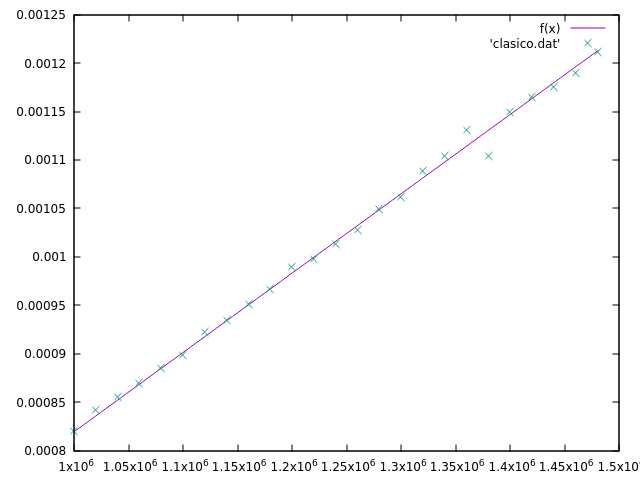
\includegraphics[scale=0.5]{hibrida_clasico.png}
\end{figure}
\end{frame}

\begin{frame}[fragile]{Algoritmo Divide y Vencerás}
\begin{figure}[H]
\centering
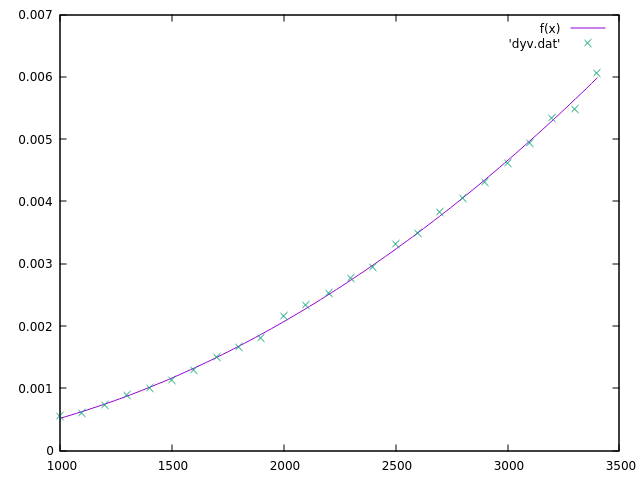
\includegraphics[scale=0.5]{hibrida_dyv.png}
\end{figure}
\end{frame}

\section*{Fin de la presentación}

\begin{frame}{Fin}
\begin{center}
\huge{Fin de la presentación}
\end{center}
\end{frame}


\end{document}


